%!TEX encoding = UTF-8 Unicode
\documentclass[french]{article}



%% Langue et compilation

\usepackage[utf8]{inputenc}
\usepackage[T1]{fontenc}
\usepackage[french]{babel}

%% LISTE DES PACKAGES

\usepackage{mathtools}     % package de base pour les maths
\usepackage{amsmath}       % mathematical type-setting
\usepackage{amssymb}       % symbols speciaux pour les maths
\usepackage{textcomp}      % symboles speciaux pour el text
\usepackage{gensymb}       % commandes generiques \degree etc...
\usepackage{tikz}          % package graphique
\usepackage{wrapfig}       % pour entourer a cote d'une figure
\usepackage{color}         % package des couleurs
\usepackage{xcolor}        % autre package pour les couleurs
\usepackage{pgfplots}      % pacakge pour creer des graph
\usepackage{epsfig}        % permet d'inclure des graph en .eps
\usepackage{graphicx}      % arguments dans includegraphics
\usepackage{pdfpages}      % permet d'insérer des pages pdf dans le document
\usepackage{subfig}        % permet de creer des sous-figure
\usepackage{pst-all}       % utile pour certaines figures en pstricks
\usepackage{lipsum}        % package qui permet de faire des essais
\usepackage{array}         % permet de faire des tableaux
\usepackage{multicol}      % plusieurs colonnes sur une page
\usepackage{enumitem}      % pro­vides user con­trol: enumerate, itemize and description
\usepackage{hyperref}      % permet de creer des hyperliens dans le document
\usepackage{lscape}        % permet de mettre une page en mode paysage
\usepackage{lmodern}       % permet d'avoir certains "fonts" de bonen qualite
\usepackage{fancyhdr}      % Permet de mettre des informations en hau et en bas de page      
\usepackage[framemethod=tikz]{mdframed} % breakable frames and coloured boxes
\usepackage[top=1.5cm, bottom=1.5cm, left=2.5cm, right=2.5cm]{geometry} % donne les marges
\usepackage[font=normalsize, labelfont=bf,labelsep=endash, figurename=Fig.]{caption} % permet de changer les legendes des figures
\usepackage{lewis}
\usepackage{bohr}
\usepackage{chemfig}
\usepackage{chemist}

%% LIBRAIRIES

\usetikzlibrary{plotmarks} % librairie pour les graphes
\usetikzlibrary{patterns}  % necessaire pour certaines choses predefinies sur tikz
\usetikzlibrary{shadows}   % ombres des encadres
\usetikzlibrary{backgrounds} % arriere plan des encadres


%% MISE EN PAGE

\pagestyle{fancy}     % Défini le style de la page

\renewcommand{\headrulewidth}{1pt}      % largeur du trait en haut de la page
\fancyhead[L]{Seconde générale}         % info coin haut gauche
\fancyhead[R]{Lycée Jean Guéhenno}  % info coin haut droit

% bas de la page
\renewcommand{\footrulewidth}{1pt}      % largeur du trait en bas de la page
\fancyfoot[L]{G. \bsc{LE DOUDIC}}  % info coin bas gauche
\fancyfoot[R]{TP 4 : Famille chimique}                         % info coin bas droit


\setlength{\columnseprule}{1pt} 
\setlength{\columnsep}{30pt}



%% NOUVELLES COMMANDES 

\DeclareMathOperator{\e}{e} % permet d'ecrire l'exponentielle usuellement


\newcommand{\gap}{\vspace{0.15cm}}   % defini une commande pour sauter des lignes
\renewcommand{\vec}{\overrightarrow} % permet d'avoir une fleche qui recouvre tout le vecteur
\newcommand{\bi}{\begin{itemize}}    % begin itemize
\newcommand{\ei}{\end{itemize}}      % end itemize
\newcommand{\bc}{\begin{center}}     % begin center
\newcommand{\ec}{\end{center}}       % end center
\newcommand\opacity{1}               % opacity 
\pgfsetfillopacity{\opacity}

\newcommand*\Laplace{\mathop{}\!\mathbin\bigtriangleup} % symbole de Laplace

\frenchbsetup{StandardItemLabels=true} % je ne sais plus

\newcommand{\smallO}[1]{\ensuremath{\mathop{}\mathopen{}o\mathopen{}\left(#1\right)}} % petit o

\newcommand{\cit}{\color{blue}\cite} % permet d'avoir les citations de couleur bleues
\newcommand{\bib}{\color{black}\bibitem} % paragraphe biblio en noir et blanc
\newcommand{\bthebiblio}{\color{black} \begin{thebibliography}} % idem necessaire sinon bug a cause de la couleur
\newcommand{\ethebiblio}{\color{black} \end{thebibliography}}   % idem
%%% TIKZ


%% COULEURS 


\definecolor{definitionf}{RGB}{220,252,220}
\definecolor{definitionl}{RGB}{39,123,69}
\definecolor{definitiono}{RGB}{72,148,101}

\definecolor{propositionf}{RGB}{255,216,218}
\definecolor{propositionl}{RGB}{38,38,38}
\definecolor{propositiono}{RGB}{109,109,109}

\definecolor{theof}{RGB}{255,216,218}
\definecolor{theol}{RGB}{160,0,4}
\definecolor{theoo}{RGB}{221,65,100}

\definecolor{avertl}{RGB}{163,92,0}
\definecolor{averto}{RGB}{255,144,0}

\definecolor{histf}{RGB}{241,238,193}

\definecolor{metf}{RGB}{220,230,240}
\definecolor{metl}{RGB}{56,110,165}
\definecolor{meto}{RGB}{109,109,109}


\definecolor{remf}{RGB}{230,240,250}
\definecolor{remo}{RGB}{150,150,150}

\definecolor{exef}{RGB}{240,240,240}

\definecolor{protf}{RGB}{247,228,255}
\definecolor{protl}{RGB}{105,0,203}
\definecolor{proto}{RGB}{174,88,255}

\definecolor{grid}{RGB}{180,180,180}

\definecolor{titref}{RGB}{230,230,230}

\definecolor{vert}{RGB}{23,200,23}

\definecolor{violet}{RGB}{180,0,200}

\definecolor{copper}{RGB}{217, 144, 88}

%% Couleur des ref

\hypersetup{
	colorlinks=true,
	linkcolor=black,
	citecolor=blue,
	urlcolor=black
		   }

%% CADRES


% %%%%%%%%%% DEFINITION
% \newmdenv[tikzsetting={fill=definitionf}, linewidth=2pt, linecolor=definitionl, outerlinewidth=0pt, innertopmargin=5pt, innerbottommargin=5pt, innerleftmargin=5pt, innerrightmargin=5pt, leftmargin=0pt]{definition}

% \newmdenv[ tikzsetting={drop shadow={ shadow xshift=1ex, shadow yshift=-0.5em, fill=definitiono, opacity=1, every shadow } }, outerlinewidth=2pt, outerlinecolor=white, linecolor=white, innertopmargin=0pt, innerbottommargin=0pt, innerleftmargin=0pt, innerrightmargin=0pt]{ombredef}


% %%%%%%%%%% THEOREME

% \newmdenv[tikzsetting={fill=theof}, linewidth=2pt, linecolor=theol, outerlinewidth=0pt, innertopmargin=5pt, innerbottommargin=5pt, innerleftmargin=5pt, innerrightmargin=5pt, leftmargin=0pt]{theo}

% \newmdenv[ tikzsetting={drop shadow={ shadow xshift=1ex, shadow yshift=-0.5em, fill=theoo, opacity=1, every shadow } }, outerlinewidth=2pt, outerlinecolor=white, linecolor=white, innertopmargin=0pt, innerbottommargin=0pt, innerleftmargin=0pt, innerrightmargin=0pt]{ombretheo}


% %%%%%%%%%% METHODE

% \newmdenv[tikzsetting={fill=metf}, linewidth=2pt, linecolor=metl, outerlinewidth=0pt, innertopmargin=5pt, innerbottommargin=5pt, innerleftmargin=5pt, innerrightmargin=5pt, leftmargin=0pt]{met}

% \newmdenv[ tikzsetting={drop shadow={ shadow xshift=1ex, shadow yshift=-0.5em, fill=meto, opacity=1, every shadow } }, outerlinewidth=2pt, outerlinecolor=white, linecolor=white, innertopmargin=0pt, innerbottommargin=0pt, innerleftmargin=0pt, innerrightmargin=0pt]{ombremet}



%%%%%%%%%%% RQ

\newmdenv[tikzsetting={fill=remf}, linewidth=2pt, linecolor=remf, outerlinewidth=0pt, innertopmargin=5pt, innerbottommargin=5pt, innerleftmargin=5pt, innerrightmargin=5pt, leftmargin=0pt]{remarque}

\newmdenv[ tikzsetting={drop shadow={ shadow xshift=1ex, shadow yshift=-0.5em, fill=remo, opacity=1, every shadow } }, outerlinewidth=2pt, outerlinecolor=white, linecolor=white, innertopmargin=0pt, innerbottommargin=0pt, innerleftmargin=0pt, innerrightmargin=0pt]{ombreremarque}

%%%%%%%%%%% Cadre pour le titre

\tikzset{every shadow/.style={opacity=1}}

\global\mdfdefinestyle{doc}{backgroundcolor=white, shadow=true, shadowcolor=propositiono, linewidth=1pt, linecolor=black, shadowsize=5pt}
\global\mdfdefinestyle{titr}{backgroundcolor=metf, shadow=true, shadowcolor=propositiono, linewidth=1pt, linecolor=black, shadowsize=5pt}
\global\mdfdefinestyle{theo}{backgroundcolor=theof, shadow=true, shadowcolor=theoo, linewidth=1pt, linecolor=theol, shadowsize=5pt}
\global\mdfdefinestyle{prop}{backgroundcolor=theof, shadow=true, shadowcolor=propositiono, linewidth=1pt, linecolor=theol, shadowsize=5pt}
\global\mdfdefinestyle{def}{backgroundcolor=definitionf, shadow=true, shadowcolor=definitiono, linewidth=1pt, linecolor=definitionl, shadowsize=5pt}
\global\mdfdefinestyle{histo}{backgroundcolor=histf, shadow=true, shadowcolor=propositiono, linewidth=1pt, linecolor=black, shadowsize=5pt}
\global\mdfdefinestyle{avert}{backgroundcolor=white, shadow=true, shadowcolor=averto, linewidth=1pt, linecolor=avertl, shadowsize=5pt}
\global\mdfdefinestyle{met}{backgroundcolor=metf, shadow=true, shadowcolor=meto, linewidth=1pt, linecolor=metl, shadowsize=5pt}
\global\mdfdefinestyle{rem}{backgroundcolor=metf, shadow=true, shadowcolor=meto, linewidth=1pt, linecolor=metf, shadowsize=5pt}
\global\mdfdefinestyle{exo}{backgroundcolor=exef, shadow=true, shadowcolor=propositiono, linewidth=1pt, linecolor=exef, shadowsize=5pt}
\global\mdfdefinestyle{not}{backgroundcolor=definitionf, shadow=true, shadowcolor=propositiono, linewidth=1pt, linecolor=black, shadowsize=5pt}
\global\mdfdefinestyle{proto}{backgroundcolor=protf, shadow=true, shadowcolor=proto, linewidth=1pt, linecolor=protl, shadowsize=5pt}

%%%%%%
\definecolor{cobalt}{rgb}{0.0, 0.28, 0.67}
\definecolor{applegreen}{rgb}{0.55, 0.71, 0.0}

\usepackage{tcolorbox}
  \tcbuselibrary{most}
  \tcbset{colback=cobalt!5!white,colframe=cobalt!75!black}



\newtcolorbox{definition}[1]{
	colback=applegreen!5!white,
  	colframe=applegreen!65!black,
	fonttitle=\bfseries,
  	title={#1}}
\newtcolorbox{Programme}[1]{
	colback=cobalt!5!white,
  	colframe=cobalt!65!black,
	fonttitle=\bfseries,
  	title={#1}}  

\newtcolorbox{Exercice}[1]{
  colback=cobalt!5!white,
  colframe=cobalt!65!black,
  fonttitle=\bfseries,
  title={#1}}  

  \newtcolorbox{Protocol}[1]{
  colback=cyan!5!white,
  colframe=cyan!65!black,
  fonttitle=\bfseries,
  title={#1}}  

\newtcolorbox{Resultat}[1]{
	colback=theof,%!5!white,
	colframe=theoo!85!black,
  fonttitle=\bfseries,
	title={#1}} 	


\def\width{12}
\def\hauteur{5}

\setlength{\parskip}{0pt}%
\setlength{\parindent}{18pt}


%% MODIFICATION DE CHAPTER  
\makeatletter
\def\@makechapterhead#1{%
  %%%%\vspace*{50\p@}% %%% removed!
  {\parindent \z@ \raggedright \normalfont
    \ifnum \c@secnumdepth >\m@ne
        \huge\bfseries \@chapapp\space \thechapter
        \par\nobreak
        \vskip 20\p@
    \fi
    \interlinepenalty\@M
    \Huge \bfseries #1\par\nobreak
    \vskip 40\p@
  }}
\def\@makeschapterhead#1{%
  %%%%%\vspace*{50\p@}% %%% removed!
  {\parindent \z@ \raggedright
    \normalfont
    \interlinepenalty\@M
    \Huge \bfseries  #1\par\nobreak
    \vskip 40\p@
  }}
  
  \newcommand{\isotope}[3]{%
     \settowidth\@tempdimb{\ensuremath{\scriptstyle#1}}%
     \settowidth\@tempdimc{\ensuremath{\scriptstyle#2}}%
     \ifnum\@tempdimb>\@tempdimc%
         \setlength{\@tempdima}{\@tempdimb}%
     \else%
         \setlength{\@tempdima}{\@tempdimc}%
     \fi%
    \begingroup%
    \ensuremath{^{\makebox[\@tempdima][r]{\ensuremath{\scriptstyle#1}}}_{\makebox[\@tempdima][r]{\ensuremath{\scriptstyle#2}}}\text{#3}}%
    \endgroup%
  }%

\makeatother

\usepackage{lewis}
\usepackage{bohr}
\usepackage{chemfig}
\usepackage{chemist}



%%% TEST EXERCIES SOLUTIONS
\usepackage{answers}
%\usepackage[nosolutionfiles]{answers}
% def d'un environnement Exercise numerote
\newtheorem{Exc}{Exercise}
\newenvironment{Ex}{\begin{Exc}\normalfont}%
                   {\end{Exc}}
% Trois types de solutions sont proposes
\Newassociation{solution}{Soln}{test}
\Newassociation{hint}{Hint}{test}
\Newassociation{Solution}{sSol}{testtwo}
\newcommand{\prehint}{~[Hint]}
\newcommand{\presolution}{~[Solution]}
\newcommand{\preSolution}{~[Homework]}
% test
\newcommand{\Opentesthook}[2]%
   {\Writetofile{#1}%
    {\protect\section{#1: #2}}}
% introduction de la solution
\renewcommand{\Solnlabel}[1]{\emph{Solution #1}}
\renewcommand{\Hintlabel}[1]{\emph{Hint #1}}
\renewcommand{\sSollabel}[1]{\emph{Solution to #1}}


%%
%%
%% DEBUT DU DOCUMENT
%%
\renewcommand{\arraystretch}{2}
\begin{document}

\tikzset{every shadow/.style={opacity=1}}

\global\mdfdefinestyle{doc}{backgroundcolor=white, shadow=true, shadowcolor=propositiono, linewidth=1pt, linecolor=black, shadowsize=5pt}
\global\mdfdefinestyle{titr}{backgroundcolor=titref, shadow=true, shadowcolor=propositiono, linewidth=1pt, linecolor=black, shadowsize=5pt}
\global\mdfdefinestyle{theo}{backgroundcolor=theof, shadow=true, shadowcolor=theoo, linewidth=1pt, linecolor=theol, shadowsize=5pt}
\global\mdfdefinestyle{prop}{backgroundcolor=theof, shadow=true, shadowcolor=propositiono, linewidth=1pt, linecolor=theol, shadowsize=5pt}
\global\mdfdefinestyle{def}{backgroundcolor=definitionf, shadow=true, shadowcolor=definitiono, linewidth=1pt, linecolor=definitionl, shadowsize=5pt}
\global\mdfdefinestyle{histo}{backgroundcolor=histf, shadow=true, shadowcolor=propositiono, linewidth=1pt, linecolor=black, shadowsize=5pt}
\global\mdfdefinestyle{avert}{backgroundcolor=white, shadow=true, shadowcolor=averto, linewidth=1pt, linecolor=avertl, shadowsize=5pt}
\global\mdfdefinestyle{met}{backgroundcolor=metf, shadow=true, shadowcolor=meto, linewidth=1pt, linecolor=metl, shadowsize=5pt}
\global\mdfdefinestyle{rem}{backgroundcolor=metf, shadow=true, shadowcolor=meto, linewidth=1pt, linecolor=metf, shadowsize=5pt}
\global\mdfdefinestyle{exo}{backgroundcolor=exef, shadow=true, shadowcolor=propositiono, linewidth=1pt, linecolor=exef, shadowsize=5pt}
\global\mdfdefinestyle{not}{backgroundcolor=definitionf, shadow=true, shadowcolor=propositiono, linewidth=1pt, linecolor=black, shadowsize=5pt}
\global\mdfdefinestyle{proto}{backgroundcolor=protf, shadow=true, shadowcolor=proto, linewidth=1pt, linecolor=protl, shadowsize=5pt}

%%%%%%

\begin{center}
	\begin{mdframed}[style=titr, leftmargin=55pt, rightmargin=55pt, innertopmargin=8pt, innerbottommargin=8pt, innerrightmargin=10pt, innerleftmargin=10pt]
		
		
		\begin{center}
			\Large{\textbf{Chapitre 2: Atome, noyau et cortège}} \medskip

			\large{\textbf{TP3: \og{}Configurations électroniques des atomes\fg{}}}
		\end{center}
	\end{mdframed}
\end{center}

% \begin{center}
% \fcolorbox{definitiono}{white}{
	
\noindent\textbf{Objectifs:}
\begin{itemize}
	\item Connaître la configuration électronique d'un atome à l'état fondamental et position dans le tableau périodique;
	\item Déterminer les électrons de valence d'un atome à partir de sa configuration fondamentale ou de sa position dans le tableau périodique.
\end{itemize}
% }
% \end{center}

\section{La configuration électronique}
	\begin{mdframed}[style=doc, leftmargin=0cm, rightmargin=0cm, innertopmargin=8pt, innerbottommargin=8pt, innerrightmargin=10pt, innerleftmargin=10pt]
		\noindent \textbf{Document 1: Composition d'un atome}\bigskip
		
		\begin{wrapfigure}{r}{.4\textwidth}
			\centering
			\vspace{-1cm}
			\includegraphics*[width=.4\textwidth]{SchemaAtome.png}
			% \caption{Schéma de l'atome}
		\end{wrapfigure}

		Un atome est constitué d'un noyau chargé positivement (contenant des protons chargés+ et des neutrons)  et d'un nuage électronique contenant des électrons.\medskip
		
		L'atome est neutre d'un point de vu électrique, il renferme autant d'électrons que de charges positives appelées protons. Ainsi que des neutrons, des particules électriquement neutres.

	\end{mdframed}


	\begin{mdframed}[style=doc, leftmargin=0cm, rightmargin=0cm, innertopmargin=8pt, innerbottommargin=8pt, innerrightmargin=10pt, innerleftmargin=10pt]
		\noindent\textbf{Document 2: La configuration électronique}\bigskip

	En 1913, le danois Niels \bsc{Bohr} propose une organisation des électrons de l'atome à l'état fondamental (non excité) en couches électroniques n = 1, 2, 3, … A l'intérieur de ces couches existent des sous-couches, notées s, p, d, …, contenant chacune un nombre limité d'électrons :\medskip


	\begin{minipage}{6cm}
	% \begin{table}[ht]
		\begin{tabular}{|c|c|}
			\hline 
			\textbf{Sous-couches} & \textbf{Nombre d'électrons} \\ \hline
			s & 2 \\ \hline
			p & 6 \\ \hline
			d & 10 \\ \hline
		\end{tabular}
	% \end{table}
	\end{minipage}\hfill
	\begin{minipage}{6cm}
		% \begin{figure}
		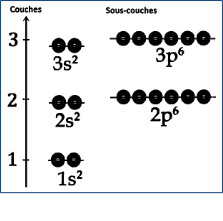
\includegraphics[width=.8\textwidth]{RemplissageSousCouchesElectroniques.jpg}
		\textbf{}
		% \caption{Remplissage maximal des sous-couches électroniques}
		% \end{figure}
	\end{minipage}

	Pour les atomes contenant moins de 18 protons (et électrons), les électrons se répartissent sur les couches électroniques s et p suivant l'ordre suivant: 
	
	\[1s\rightarrow 2s \rightarrow 2p \rightarrow 3s \rightarrow 3p\]

	\textbf{La dernière couche occupée est appelée couche de valence. Les électrons de cette couche sont appelés électrons de valence.}
\end{mdframed}

\noindent\textbf{Questions:}\medskip

\begin{enumerate}
\item Combien d'électrons trouve-t-on au maximum sur la couche 1 ? sur la couche 2 ? 

\textbf{Solution:} sur la couche 1, on trouve 2 électrons au maximum. Sur la couche 2 on trouve 8 électrons maximum.

\item Un élément possède 13 électrons, sa configuration électronique est la suivante : $1s^22s^22p^63s^23p^1$. De quel atome du tableau périodique (en annexe) il s'agit ?

\textbf{Solution:} Il s'agit de l'Aluminium.

\item Quelle sous-couche électronique correspond à ses \underline{électrons de valences} ?

\textbf{Solution:} La couche numéro 3 est la couche extérieur.

% \item Donner la configuration électronique de l'atome d'oxygène (8 électrons). Indiquer les électrons de valence. 
\end{enumerate}

% \textbf{Solution:} Il faut placer les 8 électrons en suivant la règle de remplissage des couches électroniques : $1s^22s^22p^4$. La couche des électrons de valence correspond à la couche numéro 2.

\section{La classification périodique des éléments}

\begin{mdframed}[style=doc, leftmargin=0cm, rightmargin=0cm, innertopmargin=8pt, innerbottommargin=8pt, innerrightmargin=10pt, innerleftmargin=10pt]

	\noindent\textbf{Document 3: l'intuition géniale de \bsc{Mendeleïev}}\medskip

	\begin{minipage}{4cm}
	En 1869, le chimiste russe Dimitri \bsc{Mendeleïev} classe les 63 éléments connus à son époque dans un tableau par masse atomique croissante et selon les analogies de leurs propriétés chimiques. Mais il faudra attendre le XX$^{\rm e}$ siècle (travaux de Niels \bsc{Bohr}) pour établir un lien entre ces propriétés et le cortège électronique des atomes correspondants.
	\end{minipage}\hspace{.5cm}
	\begin{minipage}{5cm}
	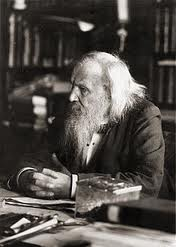
\includegraphics[width=.9\textwidth]{Mendeleiev.png}
	\end{minipage}\hfill
	\begin{minipage}{6cm}
		\centering
		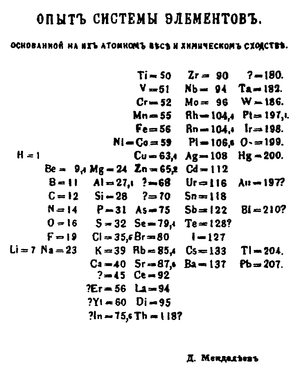
\includegraphics[width=1\textwidth]{TableauMendeleiev.png}
	\end{minipage}
\end{mdframed}


\begin{mdframed}[style=doc, leftmargin=0cm, rightmargin=0cm, innertopmargin=8pt, innerbottommargin=8pt, innerrightmargin=10pt, innerleftmargin=10pt]
\noindent\textbf{Document 4: Tableau périodique simplifié à compléter}\medskip
\begin{center}
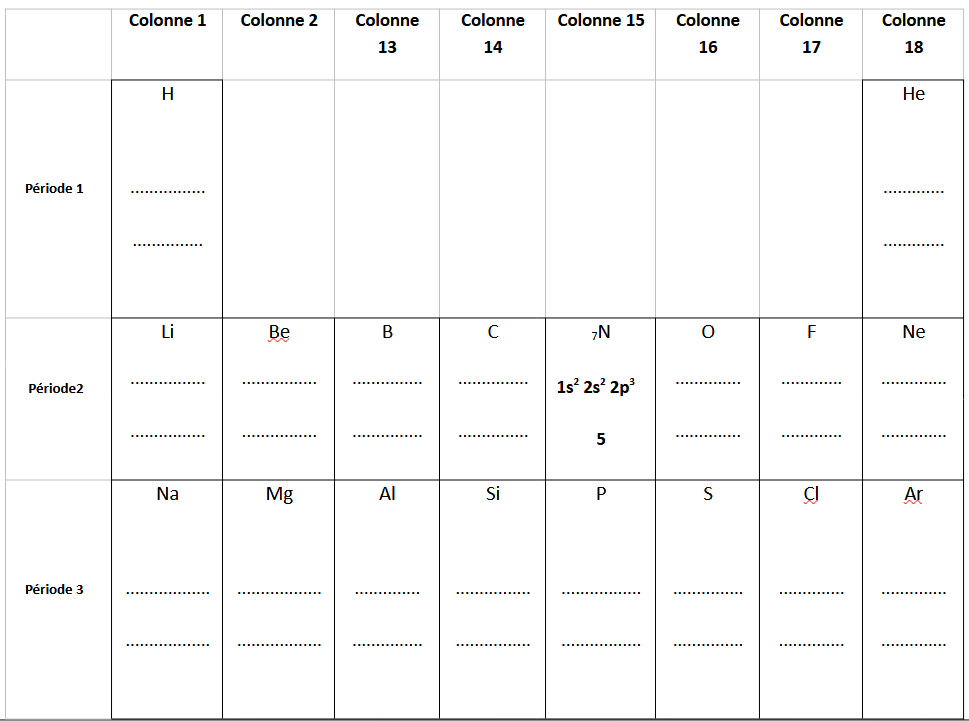
\includegraphics[width=1\textwidth]{TableauCompleter.png}
\end{center}
\end{mdframed}
\clearpage
\noindent\textbf{Questions:}\medskip
\begin{enumerate}
	\item Se connecter au site \url{www.ptable.com} pour visualiser le tableau interactif Ptable. Comparer le tableau historique de Mendeleïev avec le tableau périodique actuel. Que constatez-vous ? 
	
	\textbf{Solution:} Il y a moins d'éléments présent dans le tableau périodique de \bsc{Mendeleïev}. De plus, on remarque que les éléments Li, Na, K, Rb, Cs sont alignés sur la même ligne. Dans la classification périodique actuelle, ces éléments sont dans une même colonne.
	De même, on voit que les éléments Mg, Al, Si, P, S, Cl sont disposés à la suite dans une même colonne. Dans la classification périodique actuelle, ceux-ci sont aussi ordonnés dans une même ligne.

	\item A votre avis, pourquoi y a -t-il des points d'interrogation (par exemple pour la masse atomique 70) ?
	
	\textbf{Solution:} \bsc{Mendeleïev} ne connaissait pas tous les éléments que nous connaissons aujourd'hui. En particulier les gaz nobles sont absent de son tableau. Ces gaz nobles qui sont classés dans la dernière colonne du tableau périodique actuel sont des gaz inertes. Ils sont très stables et donc intéragissent très peu avec la matière. Il est difficile de les repérer. C'est en 1898 qu'ils ont été mis en évidence par les travaux de W. \bsc{Ramsay} et M.W. \bsc{Traverse}. En revanche les \og{}?\fg{} montre que \bsc{Mendeleïev} avait prévu l'existence de certains atomes encore inconnu en 1869.

	\item Sélectionner l'onglet \og{}Electrons\fg{}. Compléter alors le tableau du Document 3, en écrivant le numéro atomique (en bas à gauche  du symbole de l'atome)  la configuration électronique et le nombre d'électrons de valence de chaque élément.
	
		\begin{figure}[ht]
		\centering
		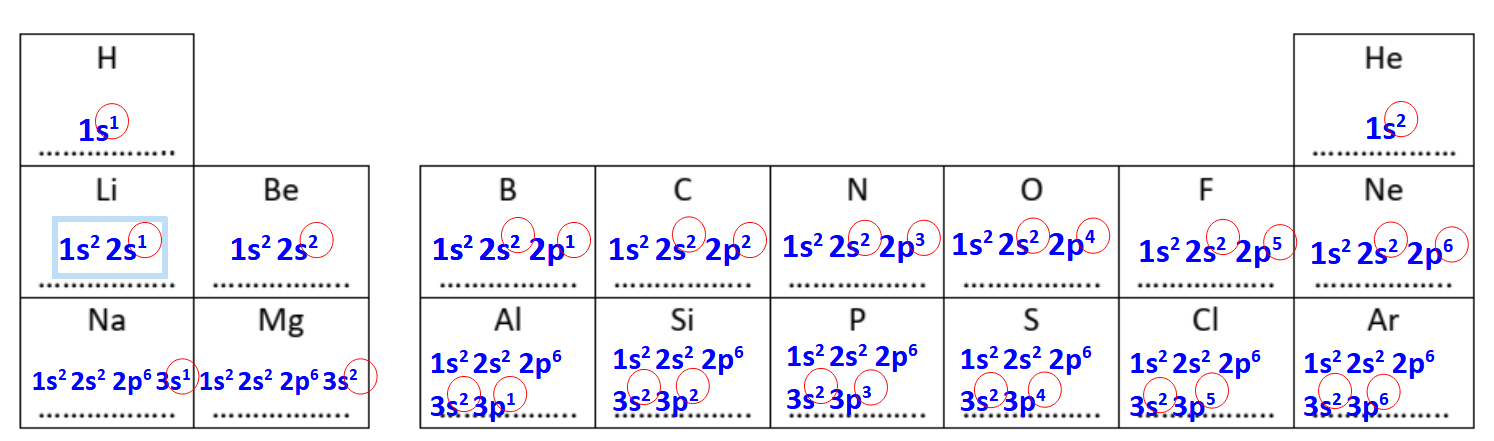
\includegraphics[width=1\textwidth]{correction.png}
	\end{figure}
	
	\item Indiquer le point commun des configurations électroniques des atomes des éléments appartenant à une même ligne, puis le point commun des configurations électroniques des atomes appartenant à une même colonne.
	
	\textbf{Solution:} Même ligne correspond au même numéro de couche électronique. Une même colonne correspond au même nombre d'électrons de valence.

	\item Déterminer la place puis le symbole de l'élément dont l'atome a pour configuration électronique : $1s^22s^22p^63s^23p^2$. Même question pour celui de configuration électronique : $1s^22s^22p^6$
	
	\textbf{Solution:}
	
	$1s^22s^22p^63s^23p^2$: l'atome est situé dans la 3e ligne (car couche 3) et dans la 14 e colonne (car 4 électrons de valence) il s agit donc du silicium Si.

	$1s^22s^22p^6$: l'atome est situé dans la 2e ligne (car couche 2) et dans la 18 e colonne (car 8 électrons de valence) il s'agit donc du néon Ne.

	\item Rédiger une règle permettant de déterminer la position d'un élément dans le tableau périodique à partir de sa configuration électronique.
	
	\textbf{Solution:} La ligne d un élément chimique correspond au numéro de la couche de valence et la colonne correspond au	nombre d électrons de valence.

	\item Dans le tableau Ptable, sélectionner l'onglet \og{}Propriétés\fg{} le nom d'une famille chimique s'affiche à gauche de l'écran. Indiquer où se trouvent les éléments appartenant aux familles chimiques suivantes : alcalins (\og{}alkali\fg{}dans le tableau), halogènes et gaz nobles.
	
	\textbf{Solution:} Les alcalins sont sur la colonne, les halogènes sur la 17eme colonne les 4 premieres lignes. Les gaz nobles sont sur la 18eme colonne.
	


	\item Sélectionner l'onglet \og{}Composés\fg{}. En sélectionnant les cases des trois premiers éléments des halogènes, compter environ combien d'associations ces atomes peuvent réaliser avec d'autres atomes. Répondre à la même question pour les trois premiers gaz nobles. Selon vous, d'où vient le terme \og{}gaz noble\fg{}?
	
	\textbf{Solution:} Tous les atomes placés dans une même colonne ont une configuration électronique similaire, c'est à dire qu'ils contiennent le même nombre d'électrons dans le même type de sous-couche électronique.

	\item Expliquer comment sont regroupés les éléments d'une même famille chimique dans le tableau périodique.
	
	\textbf{Solution:} Les éléments d'une même famille sont placés sur la même colonne du tableau périodique.

	\item Etablir un lien entre la stabilité chimique des gaz nobles et le nombre d'électrons de valence de leurs atomes. 
	
	\textbf{Solution:} Les gaz nobles sont des éléments stables car ils possèdent une couche de valence qui est remplie, s aturé e en électrons.
\end{enumerate}

% \clearpage


% \section*{1. Questions}
% \begin{enumerate}
% \item Combien d'électrons trouve-t-on au maximum sur la couche 1 ? sur la couche 2 ? 

% \textbf{Solution:} sur la couche 1, on trouve 2 électrons au maximum. Sur la couche 2 on trouve 8 électrons maximum.

% \item Un élément possède 13 électrons, sa configuration électronique est la suivante : $1s^22s^22p^63s^23p^1$. De quel atome du tableau périodique (en annexe) il s'agit ?

% \textbf{Solution:} Il s'agit de l'Aluminium.

% \item Quelle sous-couche électronique correspond à ses \underline{électrons de valences} ?

% \textbf{Solution:} La couche numéro 3 est la couche extérieur.
% \end{enumerate}
% % \item Donner la configuration électronique de l'atome d'oxygène (8 électrons). Indiquer les électrons de valence. 
% % \end{enumerate}

% % \textbf{Solution:} Il faut placer les 8 électrons en suivant la règle de remplissage des couches électroniques : $1s^22s^22p^4$. La couche des électrons de valence correspond à la couche numéro 2.


% \section*{2. Questions}

% \begin{enumerate}
% 	\item Se connecter au site \url{www.ptable.com} pour visualiser le tableau interactif Ptable. Comparer le tableau historique de Mendeleïev avec le tableau périodique actuel. Que constatez-vous ? 
	
% 	\textbf{Solution:} Il y a moins d'éléments présent dans le tableau périodique de \bsc{Mendeleïev}. De plus, on remarque que les éléments Li, Na, K, Rb, Cs sont alignés sur la même ligne. Dans la classification périodique actuelle, ces éléments sont dans une même colonne.
% 	De même, on voit que les éléments Mg, Al, Si, P, S, Cl sont disposés à la suite dans une même colonne. Dans la classification périodique actuelle, ceux-ci sont aussi ordonnés dans une même ligne.

% 	\item A votre avis, pourquoi y a -t-il des points d'interrogation (par exemple pour la masse atomique 70) ?
	
% 	\textbf{Solution:} \bsc{Mendeleïev} ne connaissait pas tous les éléments que nous connaissons aujourd'hui. En particulier les gaz nobles sont absent de son tableau. Ces gaz nobles qui sont classés dans la dernière colonne du tableau périodique actuel sont des gaz inertes. Ils sont très stables et donc intéragissent très peu avec la matière. Il est difficile de les repérer. C'est en 1898 qu'ils ont été mis en évidence par les travaux de W. \bsc{Ramsay} et M.W. \bsc{Traverse}. En revanche les \og{}?\fg{} montre que \bsc{Mendeleïev} avait prévu l'existence de certains atomes encore inconnu en 1869.

% 	\item Sélectionner l'onglet \og{}Electrons\fg{}. Compléter alors le tableau du Document 3, en écrivant le numéro atomique (en bas à gauche  du symbole de l'atome)  la configuration électronique et le nombre d'électrons de valence de chaque élément.
% 	\item Indiquer le point commun des configurations électroniques des atomes des éléments appartenant à une même ligne, puis le point commun des configurations électroniques des atomes appartenant à une même colonne.
	
% 	\begin{figure}[ht]
% 		\centering
% 		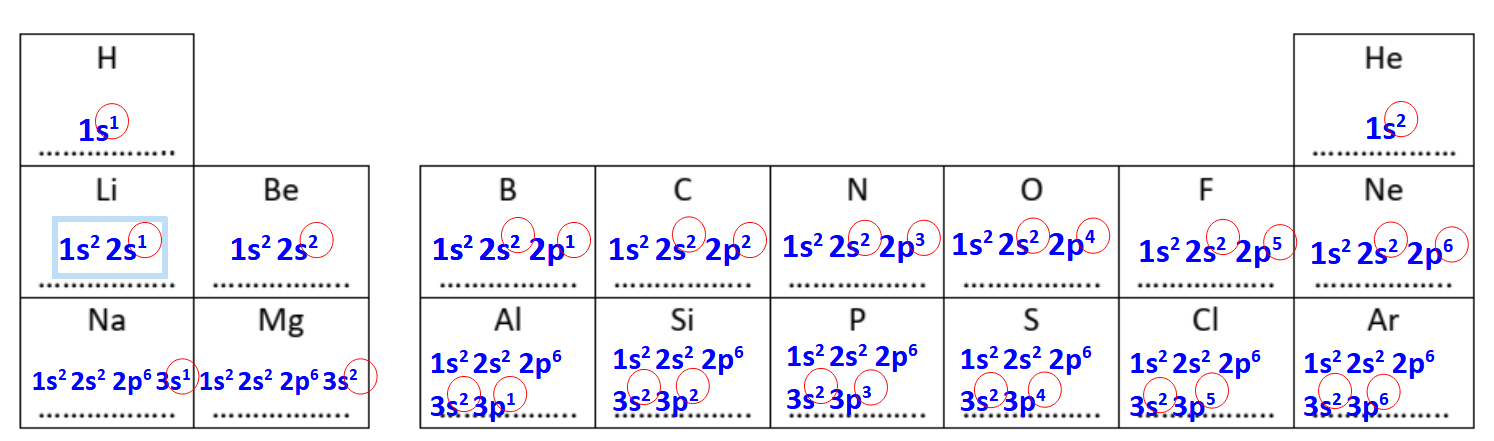
\includegraphics[width=1\textwidth]{correction.png}
% 	\end{figure}

% 	\item Déterminer la place puis le symbole de l'élément dont l'atome a pour configuration électronique : $1s^22s^22p^63s^23p^2$. Même question pour celui de configuration électronique : $1s^22s^22p^6$
	
% 	\textbf{Solution:}
	
% 	$1s^22s^22p^63s^23p^2$: l'atome est situé dans la 3e ligne (car couche 3) et dans la 14 e colonne (car 4 électrons de valence) il s agit donc du silicium Si.

% 	$1s^22s^22p^6$: l'atome est situé dans la 2e ligne (car couche 2) et dans la 18 e colonne (car 8 électrons de valence) il s'agit donc du néon Ne.

% 	\item Rédiger une règle permettant de déterminer la position d'un élément dans le tableau périodique à partir de sa configuration électronique.
	
% 	\textbf{Solution:} La ligne d un élément chimique correspond au numéro de la couche de valence et la colonne correspond au	nombre d électrons de valence.

% 	\item Dans le tableau Ptable, sélectionner l'onglet \og{}Propriétés\fg{} le nom d'une famille chimique s'affiche à gauche de l'écran. Indiquer où se trouvent les éléments appartenant aux familles chimiques suivantes : alcalins (\og{}alkali\fg{}dans le tableau), halogènes et gaz nobles.
	
% 	\textbf{Solution:} Les alcalins sont sur la colonne, les halogènes sur la 17eme colonne les 4 premieres lignes. Les gaz nobles sont sur la 18eme colonne.
	

% 	\item Sélectionner l'onglet \og{}Composés\fg{}. En sélectionnant les cases des trois premiers éléments des halogènes, compter environ combien d'associations ces atomes peuvent réaliser avec d'autres atomes. Répondre à la même question pour les trois premiers gaz nobles. Selon vous, d'où vient le terme \og{}gaz noble\fg{}?
	
% 	\textbf{Solution:} Tous les atomes placés dans une même colonne ont une configuration électronique similaire, c'est à dire qu'ils contiennent le même nombre d'électrons dans le même type de sous-couche électronique.

% 	\item Expliquer comment sont regroupés les éléments d'une même famille chimique dans le tableau périodique.
	
% 	\textbf{Solution:} Les éléments d'une même famille sont placés sur la même colonne du tableau périodique.

% 	\item Etablir un lien entre la stabilité chimique des gaz nobles et le nombre d'électrons de valence de leurs atomes. 
	
% 	\textbf{Solution:} Les gaz nobles sont des éléments stables car ils possèdent une couche de valence qui est remplie, s aturé e en électrons.
% \end{enumerate}

\end{document}

%%
%% FIN DU DOCUMENT
%%
